\appendix
\section{Additional Training Runs}

\begin{figure}[p]
    \centering
    \subfloat[Test accuracy]{
      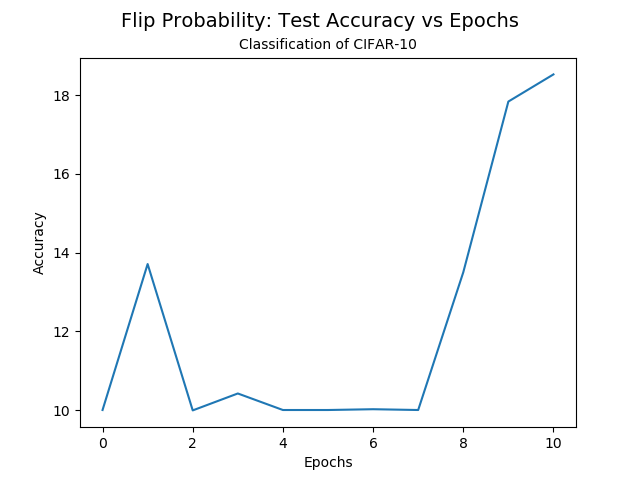
\includegraphics[width=65mm]{figs/cifar/run_1/test_accuracy_fp.png}
    }
    \subfloat[Flip probability loss - Test ]{
      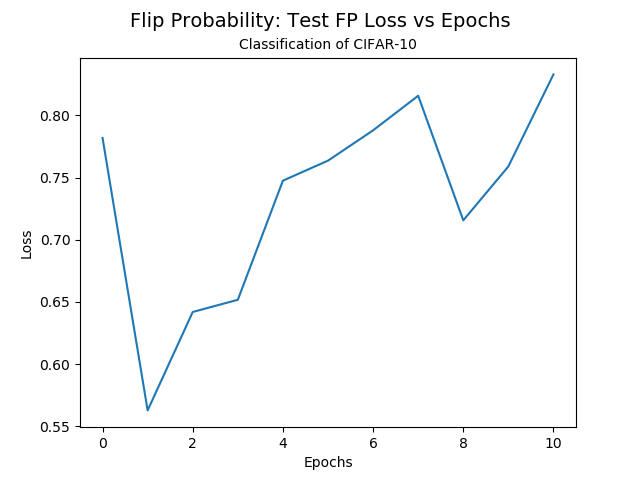
\includegraphics[width=65mm]{figs/cifar/run_1/test_losses_fp.png}
    }
    \hspace{0mm}
    \subfloat[Training accuracy]{
      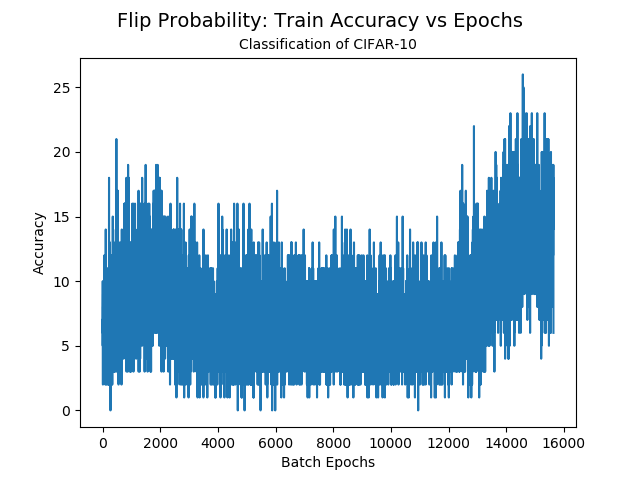
\includegraphics[width=65mm]{figs/cifar/run_1/train_accuracy.png}
    }
    \subfloat[Cross entropy loss]{
      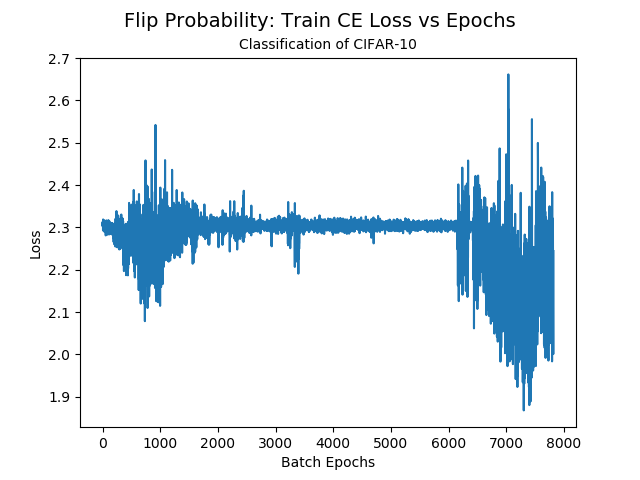
\includegraphics[width=65mm]{figs/cifar/run_1/train_losses_ce.png}
    }
    \hspace{0mm}
    \hbox to 67.5mm{}% !!
    \subfloat[Flip probability loss - training]{   % ???
      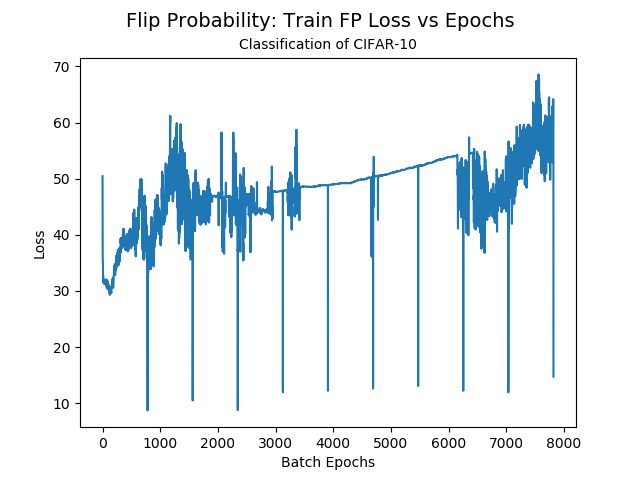
\includegraphics[width=65mm]{figs/cifar/run_1/train_losses_fp.png}
    }
    \caption[The results of the initial training scheme for CIFAR-10.]{The results of the initial training scheme, showing that the same problem of instability and poor accuracy remains.}
    \label{fig:cifar_training_scheme_1}
\end{figure}

% Insert 500 epoch graphs here, and CIFAR once/if you get running

The \gls{hyperparameter}s for the first CIFAR-10 training scheme were;

\begin{itemize}
    \item Learning rate = 0.01
    \item Batch size = 64
    \item Momentum = 0
    \item Optimiser = Stochastic Gradient Descent
    \item Normalisation = 0.5 for mean and standard deviation across all input channels
\end{itemize}